\section{完整预处理结果与探索图}\label{app:diagnostics}
表\ref{tab:holdout-all}给出42配置在开发/B的84行指标，均为固定配置的已知集合评价，不以其中最低B分数重新选型。自动缺失指示及PCA维数取决于拟合部分，420个折的维数与误差保存在相应结果表中，不统一指定为探索中的29维。
\begingroup
\small
\renewcommand{\arraystretch}{1.08}
\setlength{\tabcolsep}{5pt}
\begin{longtable}{lrrrrrr}
\caption{固定模型所有处理在开发/B的完整指标}\label{tab:holdout-all}\\
\toprule
集合 & 模型 & 处理 & MSE & RMSE & MAE & $R^2$ \\
\midrule
\endfirsthead
\caption[]{固定模型所有处理在开发/B的完整指标（续）}\\
\toprule
集合 & 模型 & 处理 & MSE & RMSE & MAE & $R^2$ \\
\midrule
\endhead
开发 & Ridge & raw & 2.287914 & 1.512585 & 0.810238 & 0.165007 \\
开发 & Ridge & scale & 2.289115 & 1.512982 & 0.807902 & 0.164568 \\
开发 & Ridge & pca & 2.496243 & 1.579950 & 0.825501 & 0.088975 \\
开发 & Ridge & scale\_pca & 2.325464 & 1.524947 & 0.812558 & 0.151303 \\
开发 & 决策树 & raw & 2.595176 & 1.610955 & 0.829650 & 0.052869 \\
开发 & 决策树 & scale & 2.595176 & 1.610955 & 0.829650 & 0.052869 \\
开发 & 决策树 & pca & 2.593023 & 1.610287 & 0.832673 & 0.053655 \\
开发 & 决策树 & scale\_pca & 2.601778 & 1.613003 & 0.846984 & 0.050459 \\
开发 & AdaBoost & raw & 2.455500 & 1.567004 & 0.808051 & 0.103845 \\
开发 & AdaBoost & scale & 2.456175 & 1.567219 & 0.809142 & 0.103598 \\
开发 & AdaBoost & pca & 2.558242 & 1.599451 & 0.847043 & 0.066348 \\
开发 & AdaBoost & scale\_pca & 2.576916 & 1.605278 & 0.837201 & 0.059533 \\
开发 & 随机森林 & raw & 2.276036 & 1.508654 & 0.786652 & 0.169341 \\
开发 & 随机森林 & scale & 2.275386 & 1.508438 & 0.786612 & 0.169579 \\
开发 & 随机森林 & pca & 2.478859 & 1.574439 & 0.814068 & 0.095319 \\
开发 & 随机森林 & scale\_pca & 2.380177 & 1.542782 & 0.804430 & 0.131334 \\
开发 & 原XGB & raw & 2.228808 & 1.492919 & 0.780951 & 0.186578 \\
开发 & 原XGB & scale & 2.228808 & 1.492919 & 0.780951 & 0.186578 \\
开发 & 原XGB & pca & 2.461235 & 1.568832 & 0.804223 & 0.101752 \\
开发 & 原XGB & scale\_pca & 2.337533 & 1.528899 & 0.804432 & 0.146898 \\
开发 & 优化XGB & raw & 2.236749 & 1.495577 & 0.782494 & 0.183680 \\
开发 & 优化XGB & scale & 2.236749 & 1.495577 & 0.782494 & 0.183680 \\
开发 & 优化XGB & pca & 2.606732 & 1.614538 & 0.841462 & 0.048651 \\
开发 & 优化XGB & scale\_pca & 2.315206 & 1.521580 & 0.799018 & 0.155046 \\
开发 & LightGBM & raw & 2.191367 & 1.480327 & 0.788751 & 0.200242 \\
开发 & LightGBM & scale & 2.191424 & 1.480346 & 0.791429 & 0.200221 \\
开发 & LightGBM & pca & 2.667651 & 1.633295 & 0.854779 & 0.026418 \\
开发 & LightGBM & scale\_pca & 2.365943 & 1.538162 & 0.816030 & 0.136529 \\
开发 & LightGBM & native & 2.211554 & 1.487129 & 0.795697 & 0.192875 \\
开发 & HistGB & raw & 2.230219 & 1.493392 & 0.785259 & 0.186063 \\
开发 & HistGB & scale & 2.233692 & 1.494554 & 0.786407 & 0.184795 \\
开发 & HistGB & pca & 2.584429 & 1.607616 & 0.839956 & 0.056791 \\
开发 & HistGB & scale\_pca & 2.285720 & 1.511860 & 0.793138 & 0.165807 \\
开发 & HistGB & native & 2.218320 & 1.489403 & 0.787738 & 0.190405 \\
开发 & 原大网络 & raw & 2.619349 & 1.618440 & 0.790811 & 0.044046 \\
开发 & 原大网络 & scale & 2.333565 & 1.527601 & 0.739419 & 0.148346 \\
开发 & 原大网络 & pca & 2.513425 & 1.585379 & 0.768613 & 0.082704 \\
开发 & 原大网络 & scale\_pca & 2.395645 & 1.547787 & 0.748050 & 0.125689 \\
开发 & 小网络 & raw & 2.883043 & 1.697953 & 0.872168 & -0.052191 \\
开发 & 小网络 & scale & 2.260269 & 1.503419 & 0.820975 & 0.175096 \\
开发 & 小网络 & pca & 3.608054 & 1.899488 & 1.138812 & -0.316790 \\
开发 & 小网络 & scale\_pca & 2.316041 & 1.521855 & 0.822817 & 0.154741 \\
B & Ridge & raw & 1.375474 & 1.172806 & 0.714380 & 0.104320 \\
B & Ridge & scale & 1.372016 & 1.171331 & 0.711438 & 0.106572 \\
B & Ridge & pca & 1.456986 & 1.207057 & 0.710259 & 0.051242 \\
B & Ridge & scale\_pca & 1.369370 & 1.170201 & 0.705186 & 0.108295 \\
B & 决策树 & raw & 1.401940 & 1.184036 & 0.680730 & 0.087086 \\
B & 决策树 & scale & 1.401940 & 1.184036 & 0.680730 & 0.087086 \\
B & 决策树 & pca & 1.517168 & 1.231734 & 0.709635 & 0.012052 \\
B & 决策树 & scale\_pca & 1.576842 & 1.255724 & 0.749767 & -0.026806 \\
B & AdaBoost & raw & 1.444966 & 1.202067 & 0.709821 & 0.059069 \\
B & AdaBoost & scale & 1.446088 & 1.202534 & 0.708552 & 0.058338 \\
B & AdaBoost & pca & 1.508366 & 1.228155 & 0.745288 & 0.017784 \\
B & AdaBoost & scale\_pca & 1.510745 & 1.229124 & 0.748463 & 0.016235 \\
B & 随机森林 & raw & 1.334292 & 1.155116 & 0.664520 & 0.131137 \\
B & 随机森林 & scale & 1.332931 & 1.154526 & 0.663986 & 0.132023 \\
B & 随机森林 & pca & 1.477213 & 1.215407 & 0.700992 & 0.038070 \\
B & 随机森林 & scale\_pca & 1.446742 & 1.202806 & 0.707142 & 0.057912 \\
B & 原XGB & raw & 1.252744 & 1.119260 & 0.648007 & 0.184240 \\
B & 原XGB & scale & 1.252744 & 1.119260 & 0.648007 & 0.184240 \\
B & 原XGB & pca & 1.459217 & 1.207981 & 0.691446 & 0.049789 \\
B & 原XGB & scale\_pca & 1.367040 & 1.169205 & 0.681433 & 0.109813 \\
B & 优化XGB & raw & 1.242601 & 1.114720 & 0.646290 & 0.190845 \\
B & 优化XGB & scale & 1.242601 & 1.114720 & 0.646290 & 0.190845 \\
B & 优化XGB & pca & 1.512826 & 1.229970 & 0.696555 & 0.014880 \\
B & 优化XGB & scale\_pca & 1.305805 & 1.142718 & 0.674523 & 0.149688 \\
B & LightGBM & raw & 1.263230 & 1.123935 & 0.655432 & 0.177411 \\
B & LightGBM & scale & 1.253797 & 1.119731 & 0.660581 & 0.183554 \\
B & LightGBM & pca & 1.630577 & 1.276941 & 0.728529 & -0.061797 \\
B & LightGBM & scale\_pca & 1.386715 & 1.177589 & 0.677011 & 0.097001 \\
B & LightGBM & native & 1.268888 & 1.126449 & 0.652933 & 0.173727 \\
B & HistGB & raw & 1.257199 & 1.121249 & 0.659121 & 0.181339 \\
B & HistGB & scale & 1.257199 & 1.121249 & 0.659120 & 0.181338 \\
B & HistGB & pca & 1.517058 & 1.231689 & 0.703089 & 0.012124 \\
B & HistGB & scale\_pca & 1.353061 & 1.163212 & 0.695379 & 0.118915 \\
B & HistGB & native & 1.265633 & 1.125004 & 0.657481 & 0.175846 \\
B & 原大网络 & raw & 1.380860 & 1.175100 & 0.648097 & 0.100814 \\
B & 原大网络 & scale & 1.299368 & 1.139898 & 0.588549 & 0.153879 \\
B & 原大网络 & pca & 1.394061 & 1.180704 & 0.627414 & 0.092217 \\
B & 原大网络 & scale\_pca & 1.334516 & 1.155213 & 0.593131 & 0.130991 \\
B & 小网络 & raw & 1.451214 & 1.204663 & 0.629196 & 0.055000 \\
B & 小网络 & scale & 1.352561 & 1.162997 & 0.668018 & 0.119241 \\
B & 小网络 & pca & 1.764104 & 1.328196 & 0.793369 & -0.148747 \\
B & 小网络 & scale\_pca & 1.369101 & 1.170086 & 0.686410 & 0.108470 \\
\bottomrule
\end{longtable}
\endgroup

\clearpage

以下图除相关热图按原计算步骤重排外，均原样提取自保存Notebook。图\ref{fig:box1}和图\ref{fig:box2}使用填补后的训练副本且混合量纲，不能据其绝对高度跨变量比较离散程度。图\ref{fig:ols-residual}和图\ref{fig:ols-qq}仅反映OLS训练拟合；图\ref{fig:correlation}仅含输入，省略过密的格内数值，完整相关矩阵随稿提供。图\ref{fig:pca-diagnostic}只描述探索输入方差。图\ref{fig:nn-inner}反映原大网络内部选择，不是开发或B的学习曲线。
\begin{figure}[htbp]
\centering
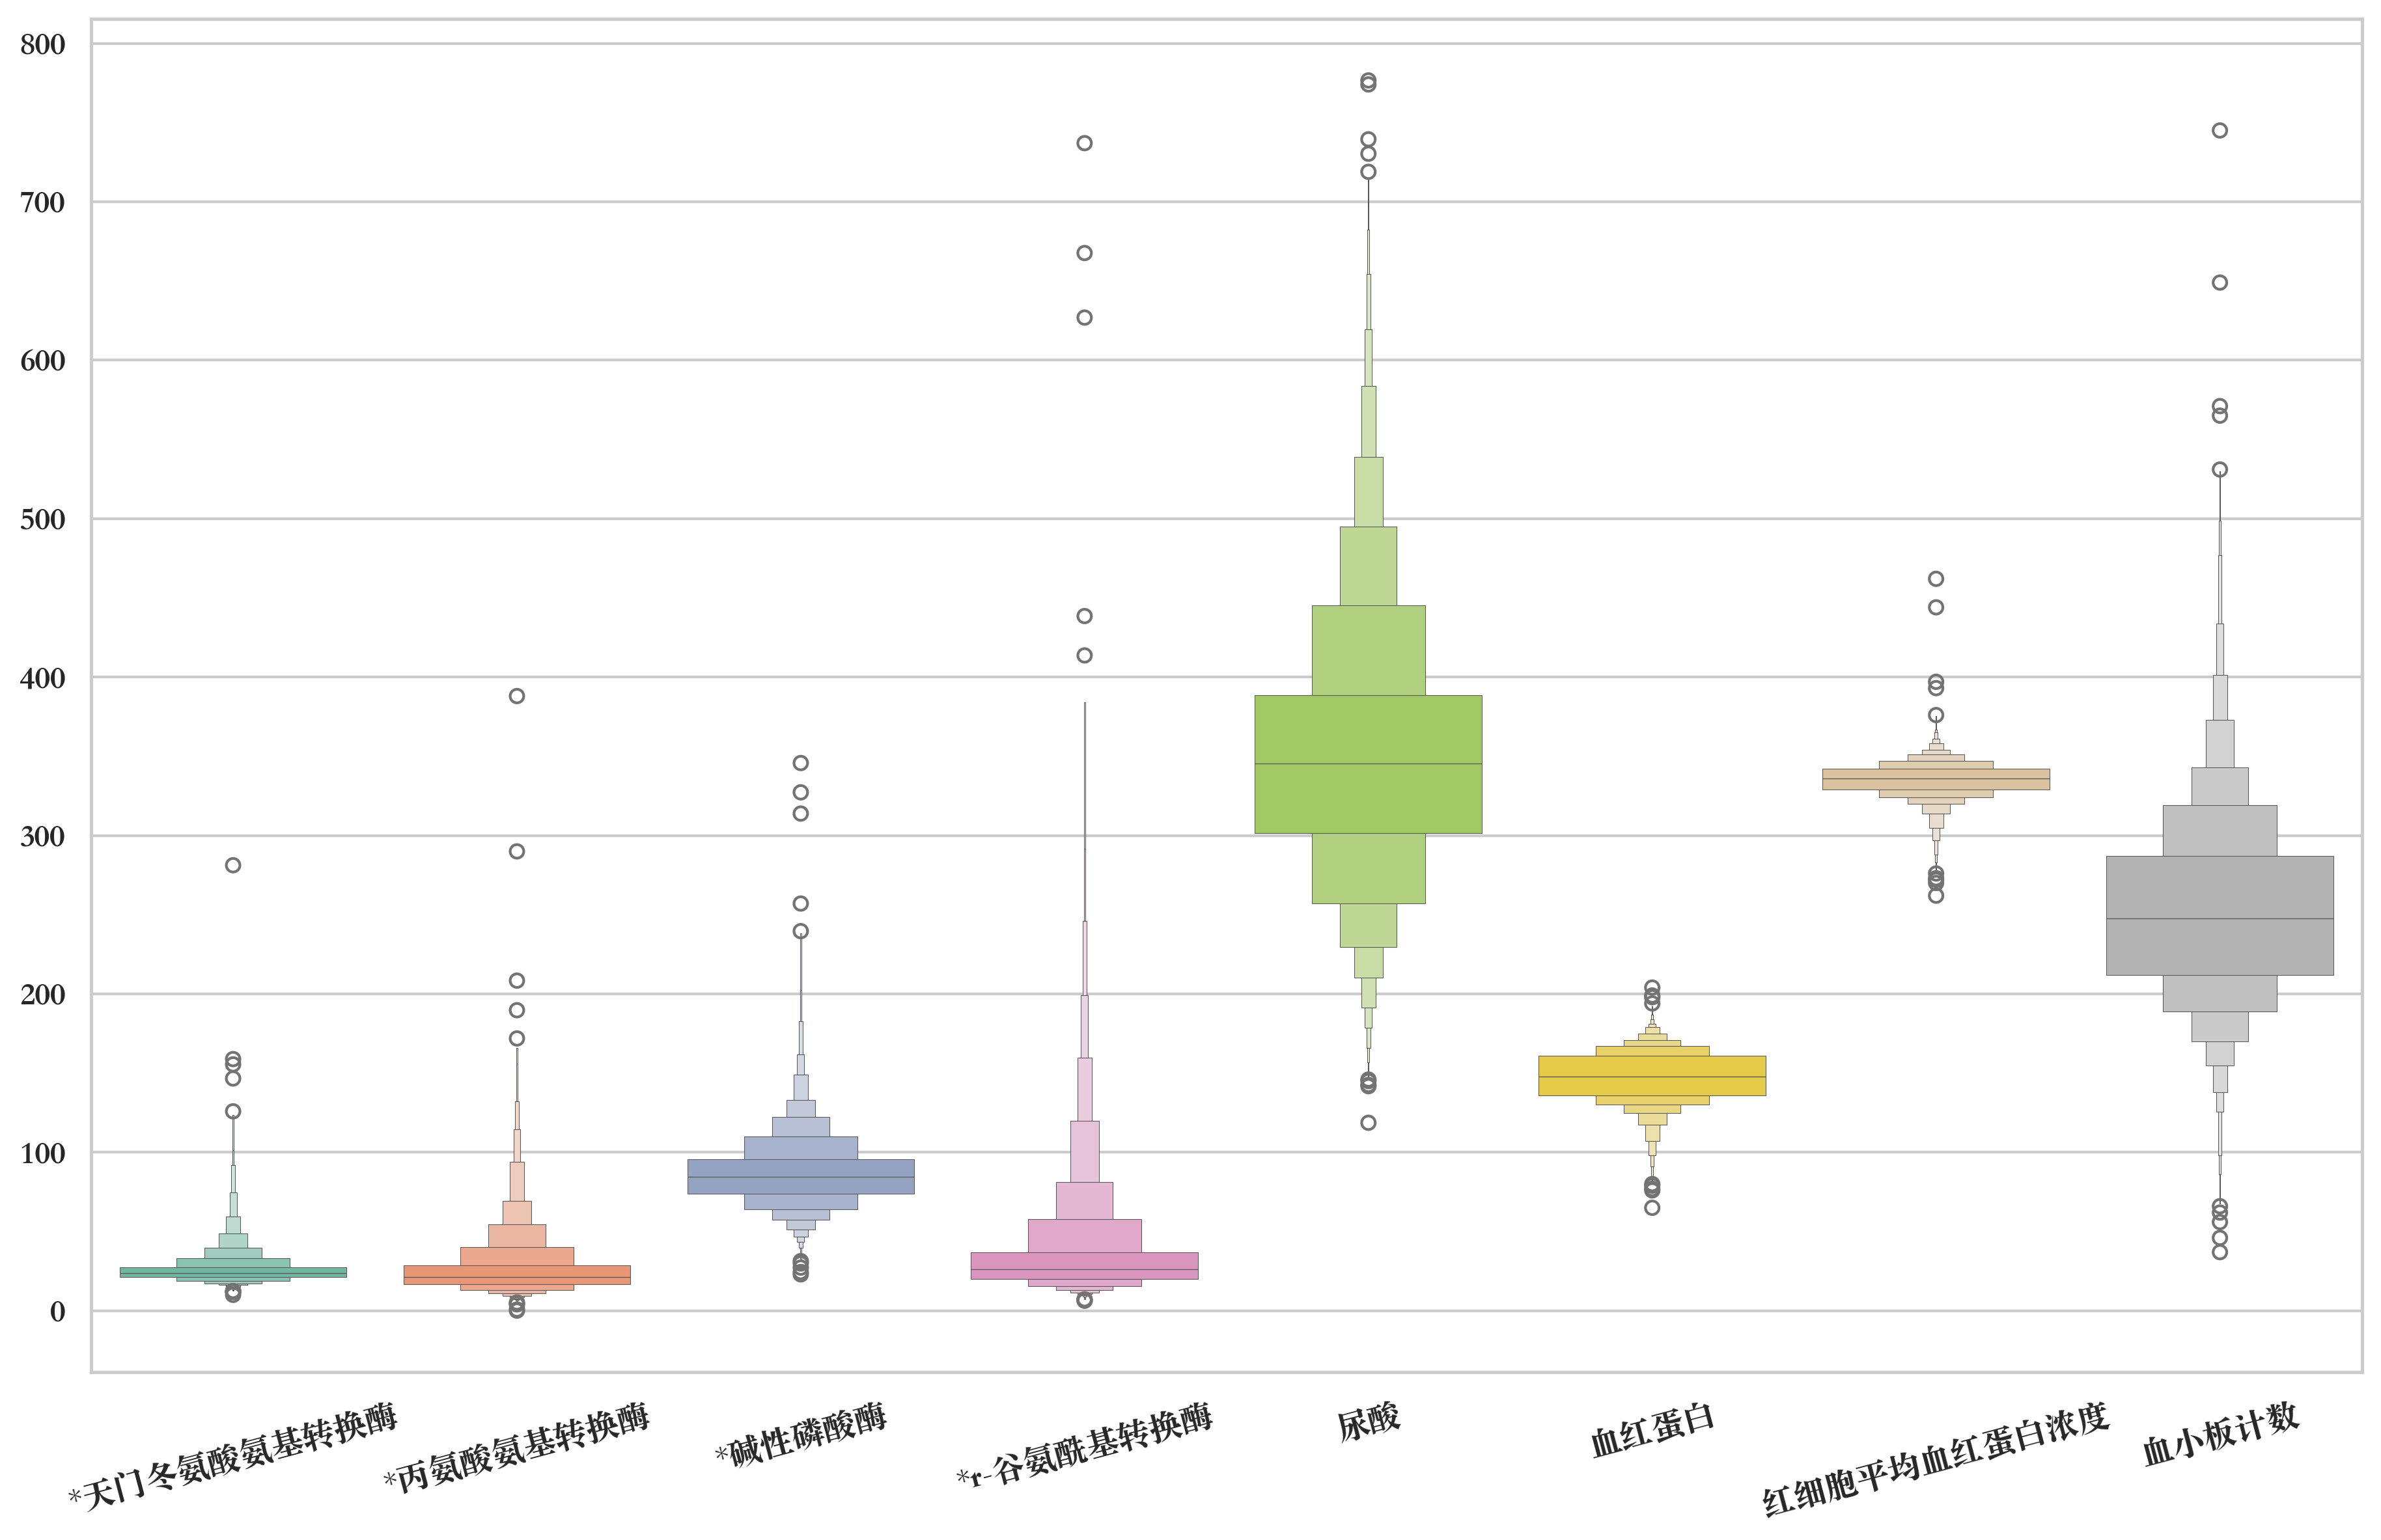
\includegraphics[width=0.94\linewidth,height=0.68\textheight,keepaspectratio]{paper/figures/paper_C026_O01.png}
\caption{训练填补副本的部分指标boxen图；指标量纲不同，图中极端记录均保留。}
\label{fig:box1}
\end{figure}
\begin{figure}[htbp]
\centering
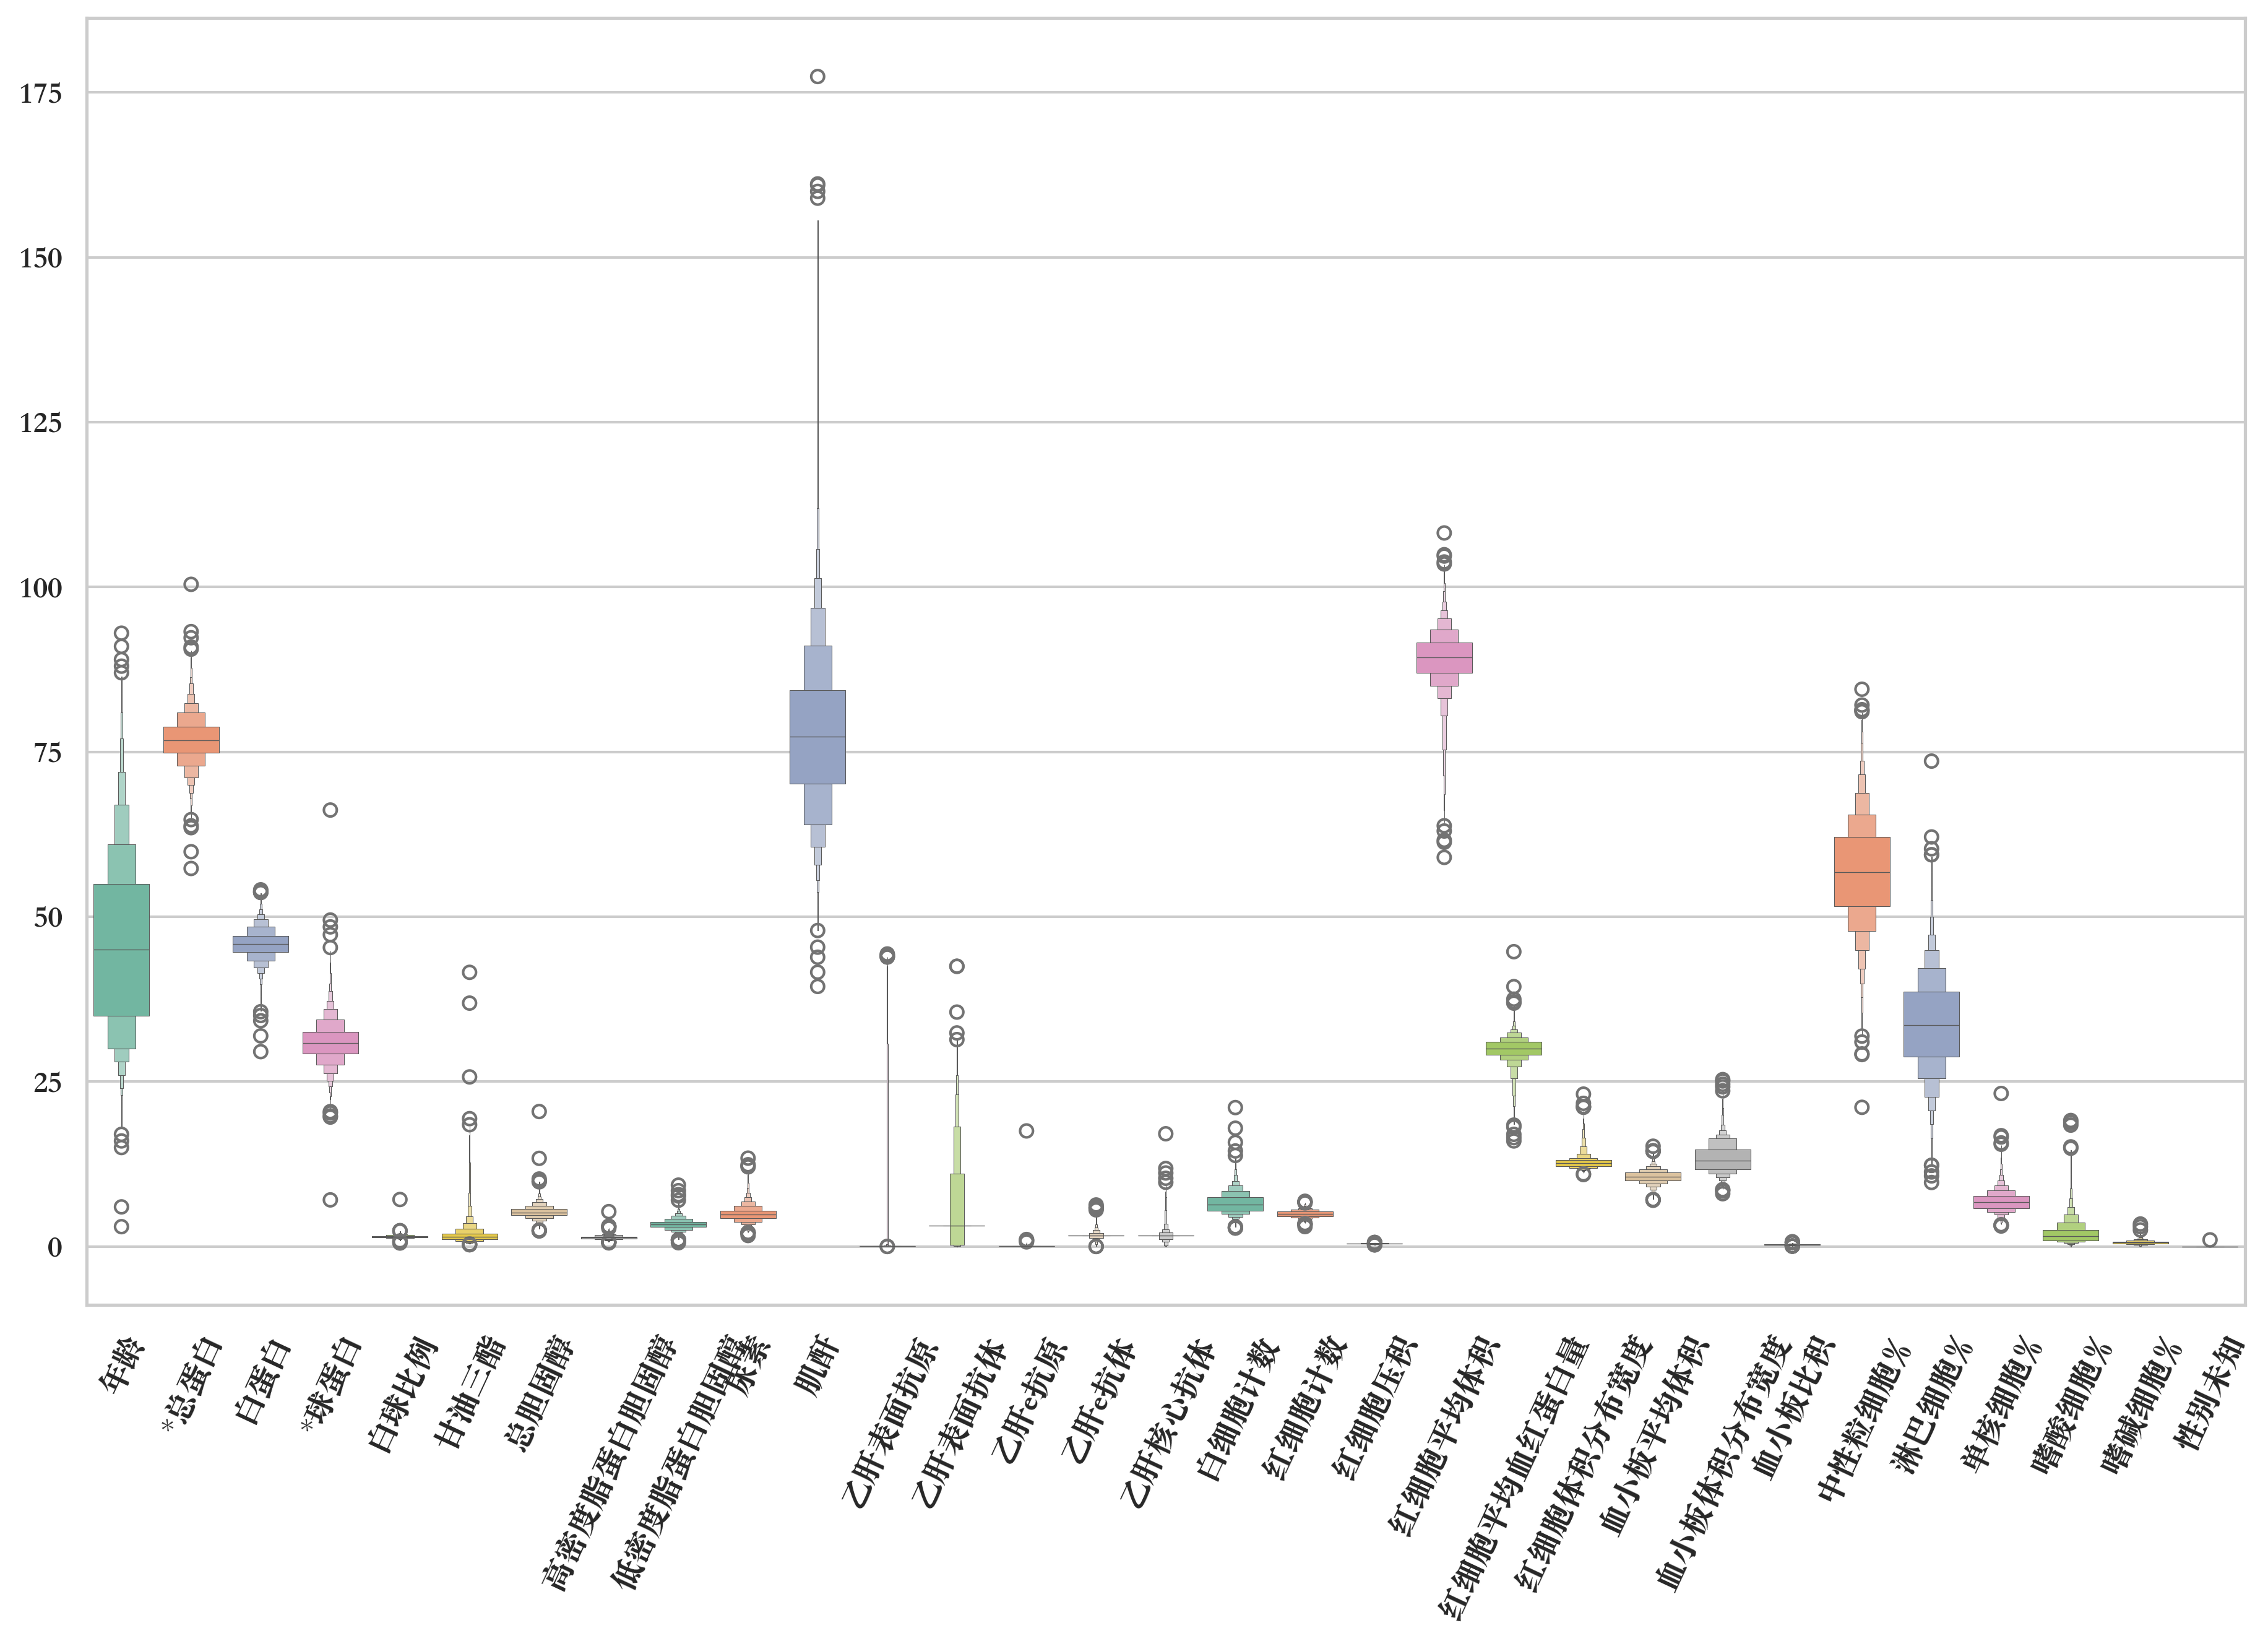
\includegraphics[width=0.94\linewidth,height=0.68\textheight,keepaspectratio]{paper/figures/paper_C027_O01.png}
\caption{训练填补副本的其余输入boxen图，包含年龄及未知指示等不同尺度变量。}
\label{fig:box2}
\end{figure}
\begin{figure}[htbp]
\centering
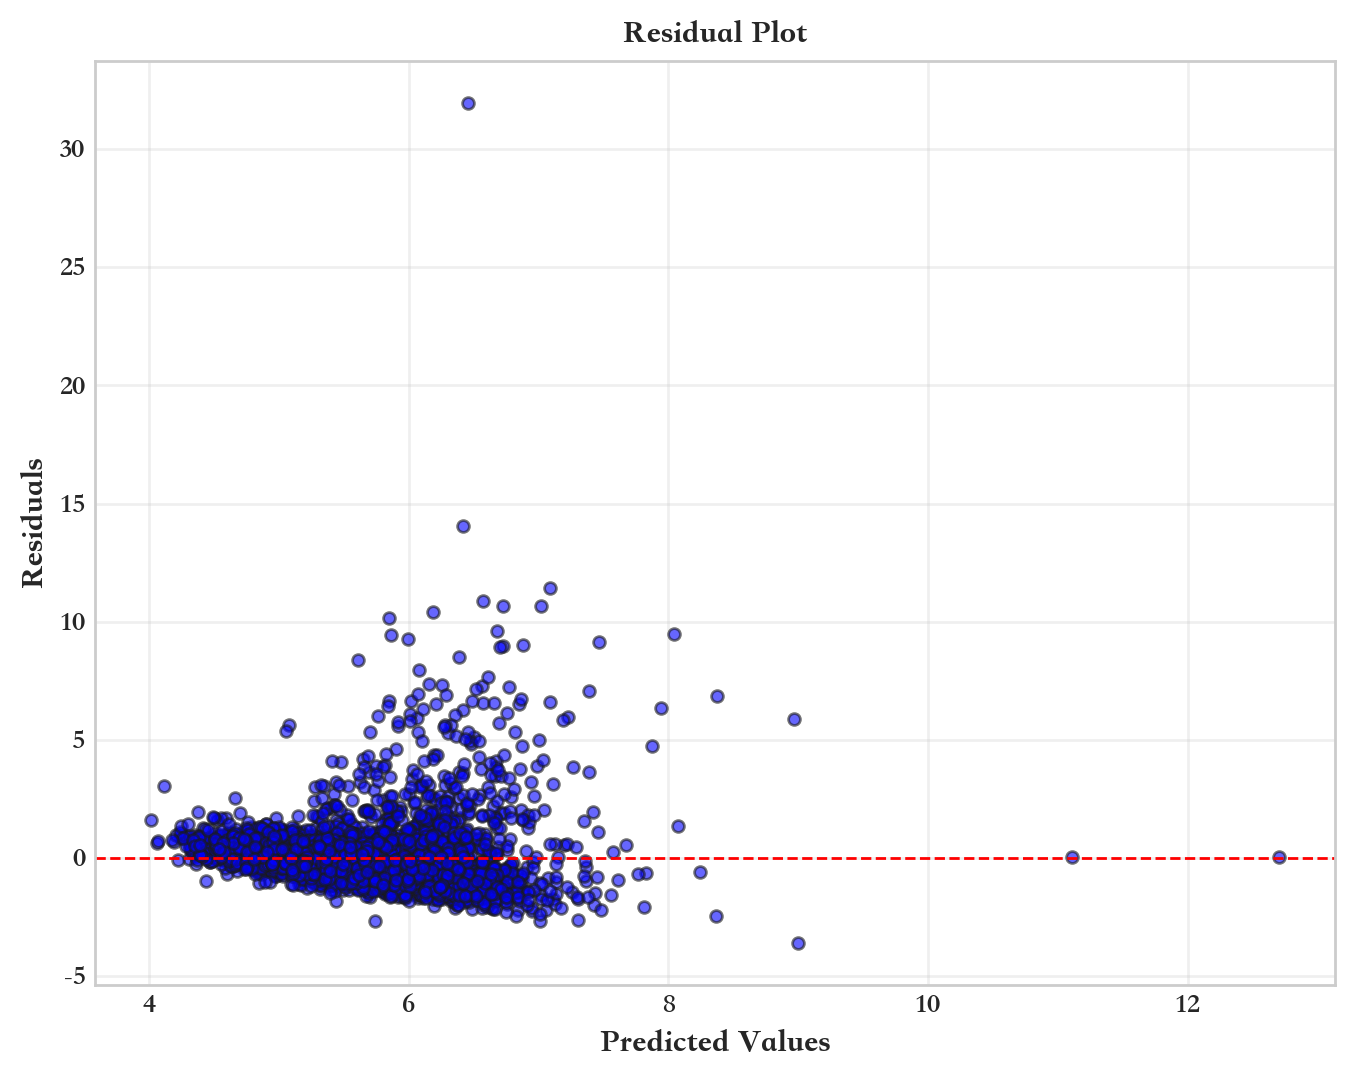
\includegraphics[width=0.94\linewidth,height=0.68\textheight,keepaspectratio]{paper/figures/paper_C032_O02.png}
\caption{OLS训练拟合残差图，不是最终融合开发或B集残差。}
\label{fig:ols-residual}
\end{figure}
\begin{figure}[htbp]
\centering
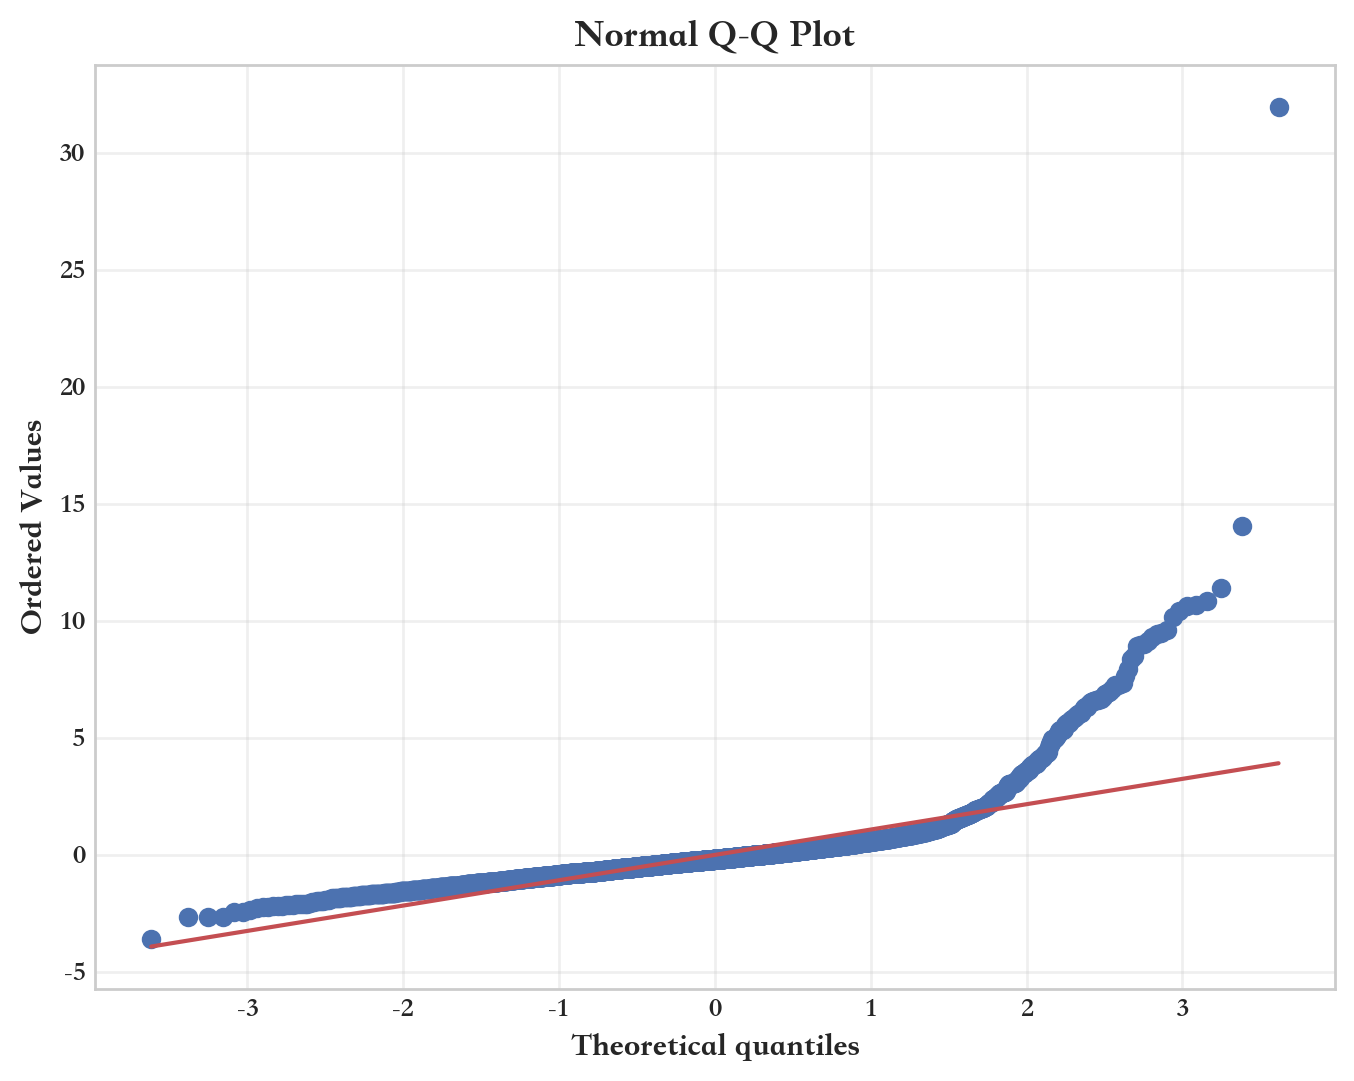
\includegraphics[width=0.94\linewidth,height=0.68\textheight,keepaspectratio]{paper/figures/paper_C032_O03.png}
\caption{OLS训练残差Q--Q图。}
\label{fig:ols-qq}
\end{figure}
\begin{figure}[p]
\centering
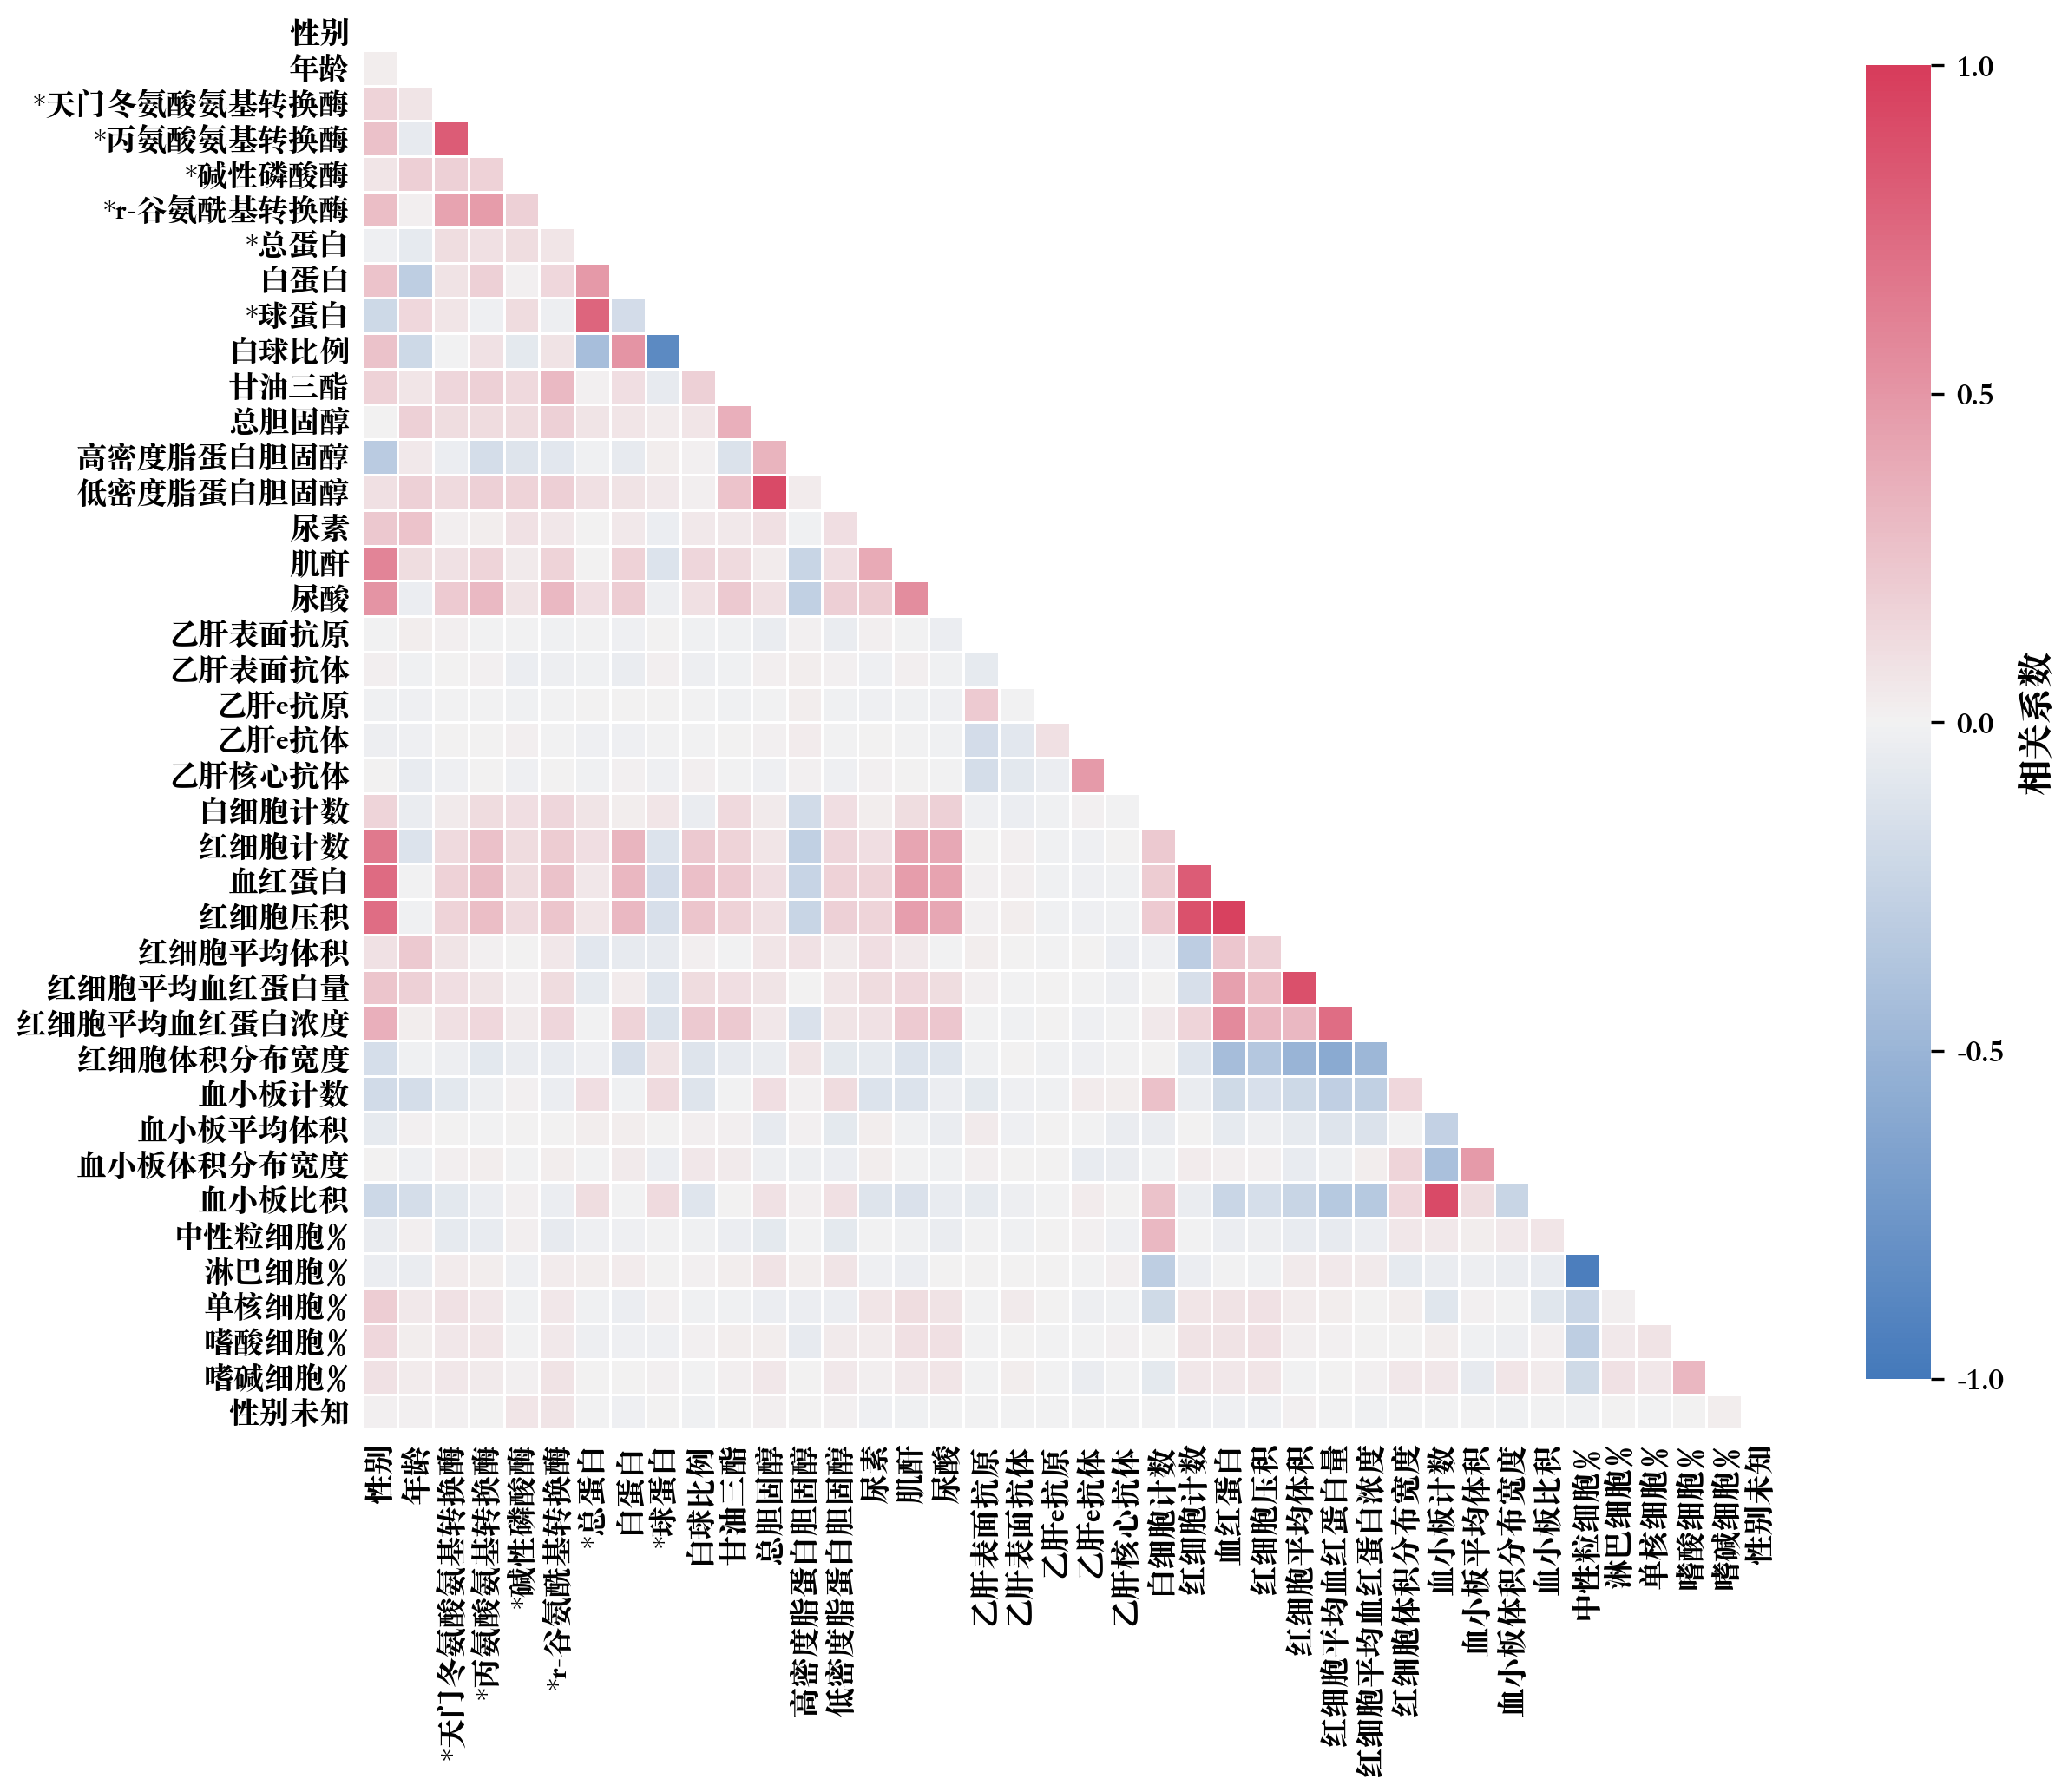
\includegraphics[width=0.94\linewidth,height=0.82\textheight,keepaspectratio]{paper/figures/training_correlation_reformatted.png}
\caption{40列训练探索输入相关热图，按原训练行与变换步骤重排；不包含血糖目标，填补及成组缺失可能影响相关结构。}
\label{fig:correlation}
\end{figure}
\begin{figure}[htbp]
\centering
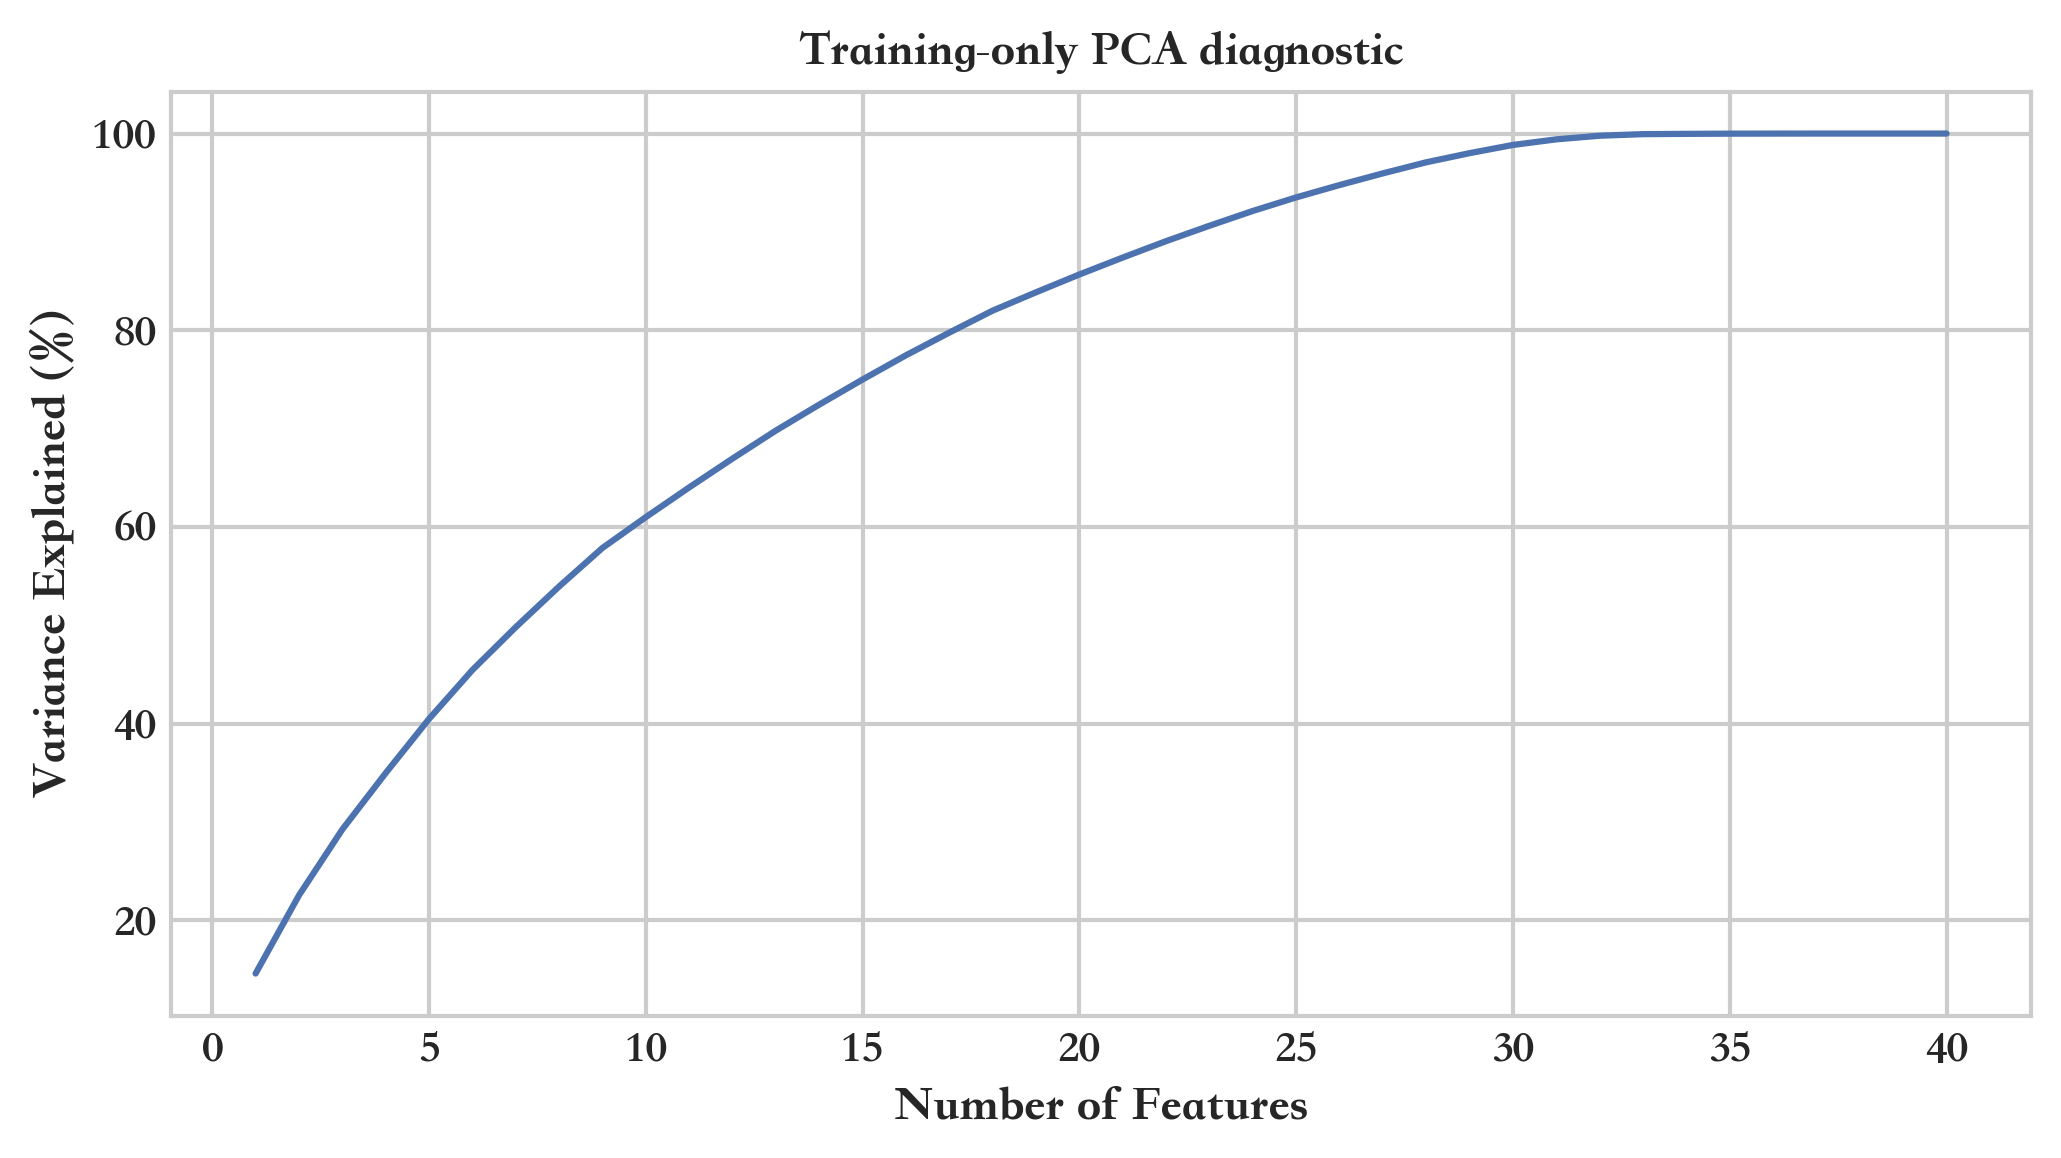
\includegraphics[width=0.94\linewidth,height=0.68\textheight,keepaspectratio]{paper/figures/paper_C040_O02.png}
\caption{训练探索矩阵的PCA累计方差；原图横轴应理解为成分序号，不是各预测折统一输入维数。}
\label{fig:pca-diagnostic}
\end{figure}
\begin{figure}[htbp]
\centering
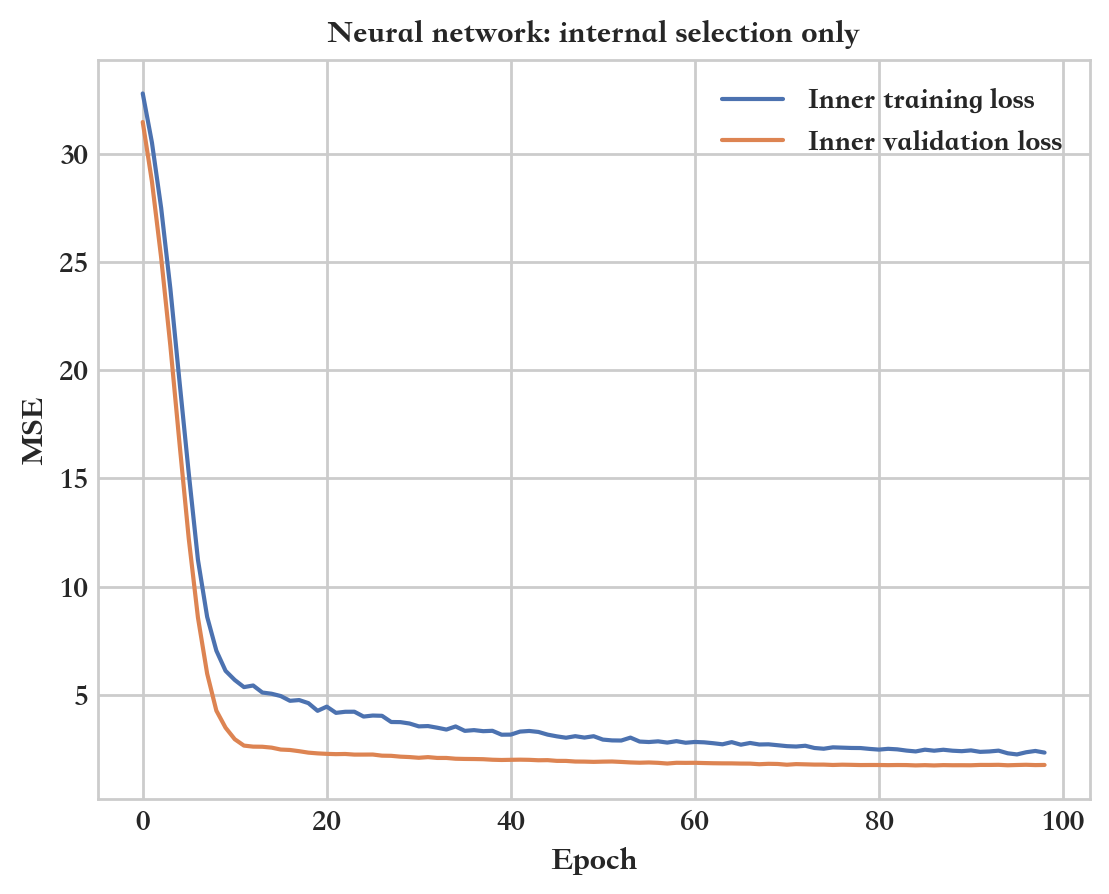
\includegraphics[width=0.94\linewidth,height=0.68\textheight,keepaspectratio]{paper/figures/paper_C051_O02.png}
\caption{原大网络内部表示与轮数选择的损失曲线；不是开发/B训练曲线。}
\label{fig:nn-inner}
\end{figure}
